\documentclass[12pt, a4paper]{article}

% --- Packages ---
\usepackage[utf8]{inputenc}
\usepackage{graphicx}
\usepackage{geometry}
\usepackage{hyperref}
\usepackage{amsmath}
\usepackage{booktabs}
\usepackage{array} % for better column formatting
\usepackage{enumitem}
\usepackage{float}
\usepackage{caption}


% --- Page setup ---
\geometry{margin=1in}

\title{\textbf{Mars Habitat Resource Recycling \& Manufacturing System}}
\author{%
    \textbf{Team Name:} Project Aurax \\[0.3em]
    \textbf{Members: }Jina Suwansirisilp, Bugra Hayrullahoglu, \\ Tianyu Ding, and Leonie Daudt 
}
\date{\today}

\begin{document}

\maketitle

\section{Problem Definition}

\subsection{Need Statement}
During a three-year mission, an eight-person crew would accumulate over 12,000 kg of inorganic waste, or trash, which is a huge problem. If the issue is not addressed as soon as possible, we humans might cause some permanent damage to the environment on Mars.

\subsection{Goal}
Find an efficient and reliable way to recycle and reuse the waste on Mars.

\subsection{Objectives}

\begin{table}[h!]
\centering
\renewcommand{\arraystretch}{1.3} % line spacing
\setlength{\tabcolsep}{8pt} % column spacing
\begin{tabular}{p{0.25\textwidth} p{0.45\textwidth} p{0.2\textwidth}}
\toprule
\textbf{Objective} & \textbf{Basis for Measurement} & \textbf{Units} \\ 
\midrule
Must be reliable & The endurance of the solution (how many years it can last) & Years \\[0.3em]
Must not be too expensive & The cost to implement the solution & CAD \\[0.3em]
Must minimize the emission & The amount of chemical the solution might emit & -- \\[0.3em]
Must be buildable by no more than eight people & Number of people required for the workload & People \\
\bottomrule
\end{tabular}
\caption{Objectives and Measurement Basis}
\end{table}

\newpage 
\subsection{Constraints}
\begin{itemize}
    \item Solutions must be completed within one week.
    \item Solutions must not burn anything without proper collection on Mars.
    \item Solutions must not cost too much money.
    \item Solutions must not be too complicated to implement.
\end{itemize}

\section{Our Solution: Mars Habitat Recycling-to-Manufacturing System (MHRMS)}

\subsection{System Overview}
\textbf{Purpose:} Convert waste materials from Mars habitat operations into usable 3D printing filament and manufacturing feedstock, with emphasis on CO2 extraction byproducts.

\textbf{Design Philosophy:} Modular, relocatable, powered by habitat grid, zero-waste discharge

\textbf{Total System Mass:} $\sim$720 kg (disassembled into $<$100 kg components)

\subsection{Mars Environment Context}
\begin{enumerate}
    \item Mars has a thin atmosphere made up mostly of carbon dioxide, nitrogen, and argon gases, with temperatures ranging from 70°F (20°C) to -225°F (-153°C)
    \item Mars' sparse atmosphere doesn't offer much protection from impacts by meteorites and the thin atmosphere causes heat from the Sun to easily escape
    \item Dust storms can cover much of the planet, sometimes taking months for all dust to settle
    \item Mars completes one rotation every 24.6 hours (a "sol"), with a year lasting 687 Earth days
    \item These conditions directly impact recycling system design: thermal management is critical, dust mitigation essential
\end{enumerate}

\subsection{Critical Mars-Specific Design Considerations}

\subsubsection{Waste Behavior in Mars Environment}
\begin{itemize}
    \item \textbf{Vacuum Exposure Challenges:} Based on NASA Glenn Research Center analysis of waste behavior when exposed to vacuum
    \item \textbf{Water Sublimation:} When waste is exposed to Mars' near-vacuum conditions (0.6\% Earth pressure), approximately 20\% of water content will sublimate before the waste completely freezes. This process takes:
    \begin{itemize}
        \item Small items (3mm droplets): $\sim$7 seconds to freeze
        \item Standard waste "football" (20cm compressed bundle): $\sim$3.4 hours to freeze
    \end{itemize}
    \item \textbf{Implications for Recycling System:}
    \begin{enumerate}
        \item Pre-processing must handle both frozen and partially sublimated materials
        \item Vapor capture systems required to prevent water loss during initial processing
        \item Grinding chambers must be sealed to capture sublimating volatiles
        \item Temperature control critical: waste arriving at facility may be frozen solid (-153°C from overnight exposure)
    \end{enumerate}
\end{itemize}

\subsubsection{Thermal Management on Mars}
\begin{itemize}
    \item \textbf{Challenge:} Mars temperature swings from 70°F (20°C) to -225°F (-153°C)
    \item \textbf{Solutions:}
    \begin{itemize}
        \item Insulated processing chambers: Maintain optimal processing temperatures (150-1400°C depending on module)
        \item Pre-heating systems: Thaw frozen waste before processing
        \item Waste heat recovery: Capture heat from processing for habitat use
        \item Phase-change thermal buffers: Smooth out temperature fluctuations
    \end{itemize}
\end{itemize}

\subsubsection{Mars Sol Adaptation}
\begin{itemize}
    \item \textbf{Mars Day:} 24.6 hours (24h 39m) vs Earth's 24 hours
    \item \textbf{Operational Impact:}
    \begin{itemize}
        \item Processing schedules calibrated to Mars sols
        \item Automation advantage: rovers and processing continue during crew sleep cycles
        \item Benefit: Extra 39 minutes per sol allows for extended processing cycles
    \end{itemize}
\end{itemize}

\noindent\textit{Source:} \href{https://science.nasa.gov/mars/facts/}{NASA Mars Facts}.

\section{Input Categories}

\begin{enumerate}
    \item \textbf{Category A -- Carbon Materials:}
    \begin{itemize}
        \item Surplus carbon from CO2 extraction (primary feedstock)
        \item Activated carbon filters (spent)
        \item Carbon-containing composites
    \end{itemize}

    \item \textbf{Category B -- Polymers/Plastics:}
    \begin{itemize}
        \item Nitrile gloves
        \item Resealable bags (PE/PP)
        \item EVA waste from spacesuits and cargo transfer bags (Nomex, nylon, polyester)
        \item Packaging materials (air cushions, bubble wrap, anti-static bags)
        \item Tape, labels, plastic clips
        \item Foam packaging (Zotek F30, Plastazote foam)
    \end{itemize}

    \item \textbf{Category C -- Fabrics:}
    \begin{itemize}
        \item Clothing (cotton, polyester, nylon)
        \item Washcloths and wipes (cellulose, cotton)
        \item Disinfectant wipes 
    \end{itemize}

    \item \textbf{Category D -- Food Packaging:}
    \begin{itemize}
        \item Overwrap materials
        \item Rehydratable pouches (polyester, polyethylene, aluminum, nylon)
        \item Drink pouches
        \item Thermal pouches
    \end{itemize}

    \item \textbf{Category E -- Metals:}
    \begin{itemize}
        \item Filter mesh (stainless steel, aluminum)
        \item Broken tools and fasteners
        \item Structural components from temporary structures
        \item Electronics casings
        \item Wire scraps
        \item Aluminum structures
    \end{itemize}

    \item \textbf{Category F -- Composites:}
    \begin{itemize}
        \item Polymer matrix composites with carbon fiber
        \item Multi-layer materials
        \item Fabric-backed materials
        \item Adhesive-bonded assemblies
    \end{itemize}
\end{enumerate}

\subsection{NASA Data Reference}
Based on ISS and shuttle waste studies, daily waste generation averages 1.45 kg per crew member, including 0.160 kg clothing, 0.352 kg food/packaging, 0.449 kg human waste, and other consumables. For a 4-person crew on a 180-day mission, this totals approximately 1,046 kg of recyclable waste.

\subsection{Sorting Protocol}
\begin{itemize}
    \item Manual inspection - crew separates by visual category
    \item Magnetic separation - ferrous vs non-ferrous metals
    \item Density sorting - polymer type identification
    \item Quality control - contamination check, damage assessment
    \item Storage: Separate sealed containers for each category in airlock staging area
\end{itemize}

\section{Alternative Waste Processing Options}

\begin{enumerate}
    \item \textbf{Option A -- Direct Venting to Space (NOT RECOMMENDED)}
    
    NASA Glenn Research Center evaluated simply disposing waste via airlock to space. Key findings:
    
    \textbf{Technical Challenges:}
    \begin{enumerate}
        \item Time-intensive: Using existing airlock technology (3-hour depressurization cycle), disposing of waste from a 180-day, 4-person mission would require 1,250-2,500 hours of crew time
        \item Hazard: 20\% of water content sublimates and can re-condense on spacecraft surfaces or contaminate equipment
        \item Trajectory risk: Low-velocity disposal at L2 libration points risks waste re-impacting spacecraft
    \end{enumerate}
    \textbf{Conclusion:} Direct disposal to space is impractical and hazardous for Mars missions

    \item \textbf{Option B: Partial Processing to Mixed Gases}
    
    NASA's "Trash-to-Gas" (TtG) Approach: Process waste in primary reactor only, producing mixed gases:
    \begin{itemize}
        \item 10\% H$_2$, 22\% CO, 68\% CO$_2$
        \item Can be used in resistojet thrusters (134.3 sec Isp)
        \item Requires 0.28 kg/crew-day makeup water
    \end{itemize}
    
    \textbf{Benefits:}
    \begin{itemize}
        \item Simpler system (fewer processing steps)
        \item Can provide station-keeping propulsion
        \item Lower energy requirements
    \end{itemize}
    
    \textbf{Limitations:}
    \begin{itemize}
        \item Lower-quality propellant (vs. pure O$_2$/CH$_4$)
        \item Still requires makeup water
        \item Limited manufacturing applications
    \end{itemize}

    \item \textbf{Option C: Full Processing to High-Quality Propellants (RECOMMENDED)}
    
    NASA's "Trash-to-Supply Gas" (TtSG) - Our Baseline: Complete processing through secondary reactors:
    \begin{itemize}
        \item 59\% O$_2$, 41\% CH$_4$ (optimal rocket propellant)
        \item Can achieve 250+ sec Isp in rocket engines
        \item Enables both propulsion AND manufacturing uses
        \item Requires 0.15 kg/crew-day makeup water (less than TtG)
    \end{itemize}
\end{enumerate}

\subsection{Our Enhanced System vs NASA's Approach}

\textbf{NASA TtSG (gases only):}
\begin{itemize}
    \item Produces O$_2$ and CH$_4$ for propulsion
    \item Vents excess gases or stores in tanks
    \item Limited to propellant applications
\end{itemize}

\textbf{Our Integrated System (gases + solids + ISRU):}
\begin{itemize}
    \item Processes waste into filament AND propellant gases
    \item Combines with regolith to create metals, glass, ceramics
    \item 3D prints replacement parts, tools, habitat components
    \item Enables true self-sufficiency vs. just propellant production
    \item Creates complete manufacturing economy
\end{itemize}

\textbf{Result:} Our system achieves everything NASA's TtSG does PLUS enables permanent settlement through manufacturing capability.

\section{System Modules}

\subsection{Module 1: Carbon Processing Station}

\textbf{Equipment Components:}
\begin{itemize}
    \item Enclosed ball mill grinder (50 kg)
    \item Compression mold press (75 kg)
    \item Electric heating elements (25 kg)
    \item Polymer binder mixing chamber (25 kg)
    \item Extrusion die set (15 kg)
    \item Control electronics (10 kg)
    \item \textbf{Total Module Mass: 200 kg}
\end{itemize}

\textbf{Process Flow:}

\textbf{Path 1A: Carbon-Composite Filament (Primary Output)}
\begin{enumerate}
    \item \textbf{Grinding:} Load carbon material into sealed ball mill, grind to 10-50 micron powder (2-4 hours)
    \item \textbf{Binder Preparation:} Shred compatible plastic waste, heat to 180-220°C
    \item \textbf{Mixing:} Ratio: 20-40\% carbon powder, 60-80\% polymer binder, blend at 200-250°C (30-60 minutes)
    \item \textbf{Extrusion:} Feed through heated barrel, extrude through 1.75mm or 2.85mm die
    \item \textbf{Spooling:} Wind onto reusable spools, label and store
\end{enumerate}

\textbf{Path 1B: Pure Carbon Products}
\begin{itemize}
    \item Activated Carbon Filters: Compress powder, heat to 800-1000°C
    \item Graphite Components: High-pressure compression, high-temperature treatment (2000-3000°C)
    \item Radiation Shielding Blocks: Mix carbon with regolith simulant
\end{itemize}

\textbf{Energy Profile:}
\begin{itemize}
    \item Power source: Habitat electrical grid
    \item Power consumption: 2-3 kW continuous
    \item Processing time: 4-8 hours per batch (5-10 kg output)
\end{itemize}

\subsection{Module 2: Polymer Recycling Station}

\textbf{Equipment Components:}
\begin{itemize}
    \item Enclosed shredder/grinder with HEPA filtration (80 kg)
    \item Multi-zone heating chamber (60 kg)
    \item Filament extruder with puller (45 kg)
    \item Diameter sensor and feedback control (8 kg)
    \item Vapor capture and carbon scrubber (35 kg)
    \item Spooling mechanism (12 kg)
    \item \textbf{Total Module Mass: 240 kg}
\end{itemize}

\textbf{Process Flow:}
\begin{enumerate}
    \item Material Preparation: Remove contaminants, cut to <10cm pieces
    \item Size Reduction: Grind to 3-8mm pellets/flakes
    \item Drying: Desiccant chamber at 60-80°C (if needed)
    \item Melting: Temperatures by polymer type (160-260°C)
    \item Filtration: Pass through 100-mesh stainless filter
    \item Extrusion: Precision gear pump, temperature-controlled barrel
    \item Cooling \& Diameter Control: Air cooling, servo-controlled puller
    \item Quality Control: Visual inspection, diameter verification
    \item Spooling: Wind onto 1 kg spools, store in sealed containers
\end{enumerate}

\textbf{Safety Systems:}
\begin{itemize}
    \item Vapor Management: Enclosed heating, carbon scrubber filtration
    \item Microplastic Control: Sealed negative-pressure chamber, HEPA filtration
\end{itemize}

\textbf{Energy Profile:}
\begin{itemize}
    \item Power consumption: 1.5-2.5 kW continuous
    \item Processing time: 6-10 hours per 5 kg batch
\end{itemize}

\subsection{Module 3: Metal Processing Station}

\textbf{Equipment Components:}
\begin{itemize}
    \item Heavy-duty metal shredder (100 kg)
    \item Induction furnace with crucible (150 kg)
    \item Wire drawing die set (40 kg)
    \item Casting molds (30 kg)
    \item Cooling system (25 kg)
    \item Metal powder atomizer (optional, 35 kg)
    \item \textbf{Total Module Mass: 380 kg (345 kg without atomizer)}
\end{itemize}

\textbf{Process Flow:}

\textbf{Path 3A: Metal Filament (Wire Drawing Method)}
\begin{enumerate}
    \item Shredding: Cut/shred metal components, separate by type
    \item Melting: Induction crucible (Al: 660°C, Cu: 1085°C, Steel: 1400-1450°C)
    \item Casting: Pour into rod molds (3-5mm diameter)
    \item Wire Drawing: Pull through progressively smaller carbide dies
    \item Quality Control: Diameter measurement, tensile testing
    \item Spooling: Wind onto spools, label
\end{enumerate}

\textbf{Alternative Paths:}
\begin{itemize}
    \item Path 3B: Metal Powder (atomization for advanced printing)
    \item Path 3C: Direct Casting (tools, fasteners, brackets)
\end{itemize}

\textbf{Energy Profile:}
\begin{itemize}
    \item Power consumption: 3-5 kW continuous, 5-7 kW peak
    \item Processing time: 8-12 hours per 3-5 kg batch
\end{itemize}

\subsection{Module 4: Integrated Manufacturing Hub}

\textbf{Equipment Components:}
\begin{itemize}
    \item FDM 3D printer (plastic/composite) (35 kg)
    \item Metal FDM printer with sintering (55 kg)
    \item Direct pellet extruder (40 kg)
    \item CNC finishing station (60 kg)
    \item Quality testing equipment (20 kg)
    \item Parts cleaning/post-processing (15 kg)
    \item \textbf{Total Module Mass: 225 kg}
\end{itemize}

\textbf{Manufacturing Capabilities:}
\begin{itemize}
    \item Plastic/Composite Printing: Uses filament from Modules 1 \& 2
    \item Metal Printing: Uses metal filament from Module 3
    \item Direct Pellet Printing: Uses pellets directly from Module 2
    \item Post-Processing: CNC milling, drilling, surface finishing
\end{itemize}

\textbf{Output Examples:}
\begin{itemize}
    \item Tools \& Equipment: Wrenches, screwdrivers, pliers, utensils
    \item Habitat Components: Storage containers, furniture, ductwork
    \item Life Support Parts: Filter housings, valves, pipe fittings
    \item Scientific Instruments: Sensor housings, sample containers
    \item EVA/Spacesuit Parts: Tool attachments, replacement clips
    \item Structural Elements: Habitat expansion, radiation shielding
\end{itemize}

\section{Supporting Systems}

\subsection{Power Distribution}
\begin{itemize}
    \item Power Source: Habitat electrical grid (nuclear/RTG or other primary power)
    \item Power Requirements:
    \begin{itemize}
        \item Module 1: 2-3 kW continuous
        \item Module 2: 1.5-2.5 kW continuous
        \item Module 3: 3-7 kW (varies with operation)
        \item Module 4: 0.5-2 kW continuous
        \item \textbf{Total system: 7.5-14.5 kW peak demand}
    \end{itemize}
\end{itemize}

\subsection{Environmental Control}
\begin{itemize}
    \item Atmosphere Management: Sealed/vented chambers, vapor capture, HEPA filtration
    \item Temperature Control: Insulation, waste heat recovery, radiator cooling
\end{itemize}

\subsection{Waste Management}
\begin{itemize}
    \item Non-Recyclable Residue: Minimal ($<$2\% of input mass), sealed storage
    \item Filter Maintenance: HEPA (quarterly), activated carbon (regenerated), metal mesh (cleaned)
\end{itemize}

\section{Operations Schedule}

\subsection{Daily Operations (Crew Time: 2-3 hours)}
\begin{itemize}
    \item Morning: Load materials, start grinding/shredding, monitor status
    \item Midday: High-temperature operations, extrusion, quality control
    \item Afternoon: Filament spooling, 3D printing, cleaning
    \item Evening/Night: Long-duration grinds, post-processing, batch planning
\end{itemize}

\subsection{Weekly Maintenance}
\begin{itemize}
    \item Clean all filters and screens
    \item Calibrate diameter sensors
    \item Inspect heating elements
    \item Test emergency shutoffs
    \item Lubricate moving parts
\end{itemize}

\subsection{Monthly Deep Maintenance}
\begin{itemize}
    \item Full system calibration
    \item Replace worn dies/components
    \item Deep clean all chambers
    \item Performance testing and logging
\end{itemize}

\section{Safety Protocols}

\subsection{Hazard Controls}
\begin{itemize}
    \item High Temperature: Thermal barriers, interlocked access, temperature alarms
    \item Moving Machinery: Emergency stops, guards, two-hand operation
    \item Electrical: Ground fault protection, enclosed components, proper labeling
    \item Air Quality: Continuous VOC monitoring, CO detection, particulate sensors
    \item Material Handling: Proper lifting techniques, anti-pinch points, spill containment
\end{itemize}

\subsection{Emergency Procedures}
\begin{itemize}
    \item Fire: CO2 extinguishers, power cutoff, evacuation
    \item Equipment Failure: Immediate shutdown, backup power, automatic cooling
    \item Contamination Release: Seal module, HEPA filtration, crew respirators
\end{itemize}

\section{Performance Metrics}

\subsection{Throughput Capacity}
\begin{itemize}
    \item Module 1 (Carbon): 5-10 kg/day composite filament, 2-5 kg/day pure carbon products
    \item Module 2 (Polymer): 5-8 kg/day plastic filament, $>$90\% Grade A/B quality
    \item Module 3 (Metal): 3-5 kg/day metal wire/rod, 1-2 kg/day metal powder
    \item Module 4 (Manufacturing): 0.5-2 kg/day finished parts, $>$85\% success rate
\end{itemize}

\subsection{Resource Recovery Rates}
\begin{itemize}
    \item Carbon: 95\%+ recovery
    \item Polymers: 85-90\% recovery
    \item Metals: 90-95\% recovery
    \item Fabrics: 70-80\% recovery
    \item Composites: 85-90\% recovery
\end{itemize}

\subsection{Mass Balance Example (Monthly)}
\begin{itemize}
    \item Inputs: 120 kg total (50 kg carbon, 35 kg plastic, 10 kg fabric, 20 kg metal, 5 kg composites)
    \item Outputs: 115 kg usable filament/feedstock/products
    \item Recovery rate: 96\%
\end{itemize}

\section{Crew Training Requirements}

\subsection{Basic Operator (All Crew - 8 hours)}
\begin{itemize}
    \item Safety protocols and PPE
    \item Material sorting and identification
    \item Basic module operation
    \item Emergency shutdown procedures
    \item Quality control basics
\end{itemize}

\subsection{Advanced Operator (Designated Personnel - 40 hours)}
\begin{itemize}
    \item Module-specific technical knowledge
    \item Maintenance procedures
    \item Repair and component replacement
    \item Process optimization
\end{itemize}

\subsection{System Manager (Mission Specialist - 80 hours)}
\begin{itemize}
    \item Full system integration
    \item Complex troubleshooting
    \item Performance analysis and reporting
    \item Modification and upgrades
\end{itemize}

\section{Technology Readiness \& Development Path}

\subsection{Current TRL Levels}
\begin{itemize}
    \item Individual processes: TRL 7-9 (proven on Earth)
    \item Integrated system: TRL 4-5 (lab demonstration)
    \item Mars-specific adaptations: TRL 3-4 (analytical/experimental proof)
\end{itemize}

\subsection{Development Phases}
\begin{enumerate}
    \item Phase 1 (Months 1-6): Earth prototype - build and test individual modules
    \item Phase 2 (Months 7-12): Integration testing - connect all modules
    \item Phase 3 (Months 13-18): Mars analog testing - deploy to Mars Desert Research Station
    \item Phase 4 (Months 19-24): Flight preparation - finalize designs for launch
    \item Phase 5 (Year 3+): Mars deployment - transport, assemble, commission
\end{enumerate}

\section{Advantages for Mars Operations}

\subsection{Resource Independence}
\begin{itemize}
    \item Reduces resupply needs from Earth by 60-80\%
    \item Creates self-sufficiency for consumables
    \item Enables mission extension without additional launches
\end{itemize}

\subsection{CO2 Utilization}
\begin{itemize}
    \item Valuable use for extraction byproduct (carbon)
    \item Closes carbon loop in life support
    \item Reduces carbon waste accumulation
\end{itemize}

\subsection{Adaptability}
\begin{itemize}
    \item Can process unexpected waste streams
    \item Creates custom tools/parts on-demand
    \item Supports mission changes and repairs
\end{itemize}

\subsection{Sustainability}
\begin{itemize}
    \item Zero-waste philosophy
    \item Minimal toxic byproducts
    \item Closed-loop atmosphere management
\end{itemize}

\subsection{Economic Benefits}
\begin{itemize}
    \item Each kg recycled saves $\sim$\$10,000 in launch costs
    \item Monthly savings: \$1,150,000 (115 kg recovered $\times$ \$10k/kg)
    \item System pays for itself in $\sim$2-3 months of operation
\end{itemize}

\section{Scalability \& Future Enhancements}

\subsection{Near-Term Upgrades}
\begin{itemize}
    \item Enhanced Material Library: Ceramics from regolith, glass from silicates, bio-composites
    \item Automation: Robotic sorting, autonomous quality control, self-optimization
    \item Advanced Manufacturing: Multi-material printing, larger build volumes, higher precision
\end{itemize}

\subsection{Long-Term Vision}
\begin{itemize}
    \item Colony Scale (100+ inhabitants): Multiple facilities, specialized production
    \item In-Situ Resource Utilization (ISRU): Process Martian regolith, extract local metals
    \item Distributed Manufacturing: Rover-mounted units, remote site fabrication
\end{itemize}

\section{Compliance Summary}

\begin{itemize}
    \item No incineration/burning - All thermal processing in controlled, non-combustion environment
    \item No toxic emissions - Closed-loop vapor capture with activated carbon filtration
    \item No PFAS generation - System avoids all fluoropolymers and fluorinated compounds
    \item No microplastic release - Sealed grinding with HEPA filtration; all particles captured
    \item No wastewater discharge - Dry processing only; minimal water use with closed-loop drying
    \item Safe for Martian environment - All processes contained; no surface contamination
    \item Crew safety prioritized - Multiple redundant safety systems; comprehensive training
    \item Minimal crew time - 2-3 hours daily operation; automated processes reduce workload
    \item Grid-powered efficiency - Uses habitat electrical supply; no separate power generation needed
    \item Water conservation - Minimal water use in drying processes only; closed-loop system
\end{itemize}

\section{Mars Material Collection Rover Fleet Design}

\subsection{Rover Types and Roles}

\begin{table}[h!]
\centering
\small
\renewcommand{\arraystretch}{1.4}
\setlength{\tabcolsep}{8pt}
\begin{tabular}{p{0.2\textwidth} p{0.35\textwidth} p{0.4\textwidth}}
\toprule
\textbf{Rover Type} & \textbf{Purpose / Role} & \textbf{Collected Material} \\
\midrule
Carbon Collector Rover & Gather carbon-based materials for composite filament and carbon products & CO\textsubscript{2} extraction byproducts, activated carbon filters, carbon dust, organic waste \\[0.5em]

Polymer/Plastic Collector Rover & Collect polymers and fabrics for Module 2 recycling & Nitrile gloves, EVA waste, PE/PP packaging, tape/labels, cotton/polyester/nylon clothing, wipes, food packaging \\[0.5em]

Metal Collector Rover & Collect metals for wire, rods, powder, and casting & Broken tools, fasteners, electronics casings, aluminum structures \\[0.5em]

Composite/Mixed Material Rover & Collect difficult-to-sort or multi-material items & Adhesive-bonded assemblies, fabric-backed composites, polymer-matrix carbon fiber \\[0.5em]

Regolith / ISRU Rover & Supply regolith for manufacturing, shielding, and carbon-regolith composites & Martian soil, regolith for ceramics, carbon-regolith mixes \\[0.5em]

Storage / Transport Rover & Transport collected materials to MHRMS modules & Any collected material \\[0.5em]

Maintenance / Inspection Rover & Check and service MHRMS modules & Tools, replacement parts, consumables \\
\bottomrule
\end{tabular}
\caption{Rover Types and Their Specific Roles in Material Collection}
\end{table}

\normalsize

\subsection{Rover Specifications and Features}

\subsubsection{Carbon Collector Rover}
\begin{itemize}
    \item Shovel/vacuum attachment for efficient collection
    \item Pressurized, sealed storage to capture fine carbon dust
    \item Automated sorting for polymer binders if present
    \item Mass: 150 kg
    \item Power: 2 kW continuous during operation
\end{itemize}

\subsubsection{Polymer/Plastic/Fabric Collector Rover}
\begin{itemize}
    \item Pre-sorting capability to remove metal bits and contamination
    \item Onboard shredding/compaction capability
    \item Closed storage system to prevent microplastic release
    \item Mass: 180 kg
    \item Power: 2.5 kW during shredding operations
\end{itemize}

\subsubsection{Metal Collector Rover}
\begin{itemize}
    \item Magnetic separation for ferrous/non-ferrous metals
    \item Insulated storage compartments
    \item Carbon-fiber polymer separation capability
    \item Mass: 200 kg
    \item Power: 3 kW during magnetic separation
\end{itemize}

\subsubsection{Composite/Mixed Material Rover}
\begin{itemize}
    \item Flexible, modular bins for varied material types
    \item Visual recognition system for proper storage categorization
    \item Pre-processing separation flags for Modules 1 \& 2
    \item Mass: 170 kg
    \item Power: 2.2 kW continuous
\end{itemize}

\subsubsection{Regolith / ISRU Rover}
\begin{itemize}
    \item Excavator with dust-mitigation storage system
    \item Precision dosing for Module 1 \& 4 applications
    \item Soil composition analysis sensors
    \item Mass: 220 kg
    \item Power: 3.5 kW during excavation
\end{itemize}

\subsubsection{Storage / Transport Rover}
\begin{itemize}
    \item Modular compartments with sealed docking interface
    \item Protection from material contamination or sublimation
    \item Adaptable to interface with all collection rovers
    \item Mass: 190 kg
    \item Power: 1.5 kW during transport
\end{itemize}

\subsubsection{Maintenance / Inspection Rover}
\begin{itemize}
    \item Light-load chassis for maneuverability
    \item Precision mobility system
    \item Robotic arm for module repair or replacement
    \item System performance monitoring and crew alerting
    \item Mass: 120 kg
    \item Power: 1.8 kW during maintenance operations
\end{itemize}

\subsection{Standard Electronics Compartment (All Rovers)}

\subsubsection{Power System}
\begin{itemize}
    \item Li-ion batteries (10-20 kWh capacity)
    \item Backup power from habitat electrical grid when docked
    \item Power distribution bus with overcurrent protection
    \item Solar charging capability for extended missions
\end{itemize}

\subsubsection{Control System}
\begin{itemize}
    \item Central CPU/microcontroller for autonomous operations
    \item Motor controllers and robotic arm interface
    \item Integration with MHRMS module scheduling software
    \item Redundant processing units for critical functions
\end{itemize}

\subsubsection{Communication Systems}
\begin{itemize}
    \item UHF/X-band relay for Mars orbital communication
    \item Inter-rover Wi-Fi mesh network
    \item Inertial + orbital localization systems
    \item Redundant communication pathways
\end{itemize}

\subsubsection{Sensor Suite}
\begin{itemize}
    \item Visual + IR cameras for navigation and inspection
    \item LiDAR for precise mapping and obstacle avoidance
    \item Material-specific sensors: CO\textsubscript{2} detection, metal sensors, dust sensors
    \item Environmental monitoring: temperature, pressure, radiation levels
\end{itemize}

\subsubsection{Autonomy \& AI}
\begin{itemize}
    \item Edge AI for autonomous path planning and material detection
    \item Machine learning algorithms for optimal collection routes
    \item Optional human override from habitat or rover hub
    \item Automated docking to MHRMS modules
\end{itemize}

\subsubsection{Safety \& Redundancy}
\begin{itemize}
    \item Thermal insulation for Mars temperature extremes (-153°C to 20°C)
    \item Overcurrent and voltage monitoring with automatic shutdown
    \item Emergency stop for all motors and robotic arms
    \item Redundant power and communication systems
\end{itemize}

\subsubsection{Storage Interface}
\begin{itemize}
    \item Modular, sealed compartments for material categories:
    \begin{itemize}
        \item Carbon materials compartment
        \item Polymers/Fabrics storage
        \item Metals collection bins
        \item Composites handling system
        \item Regolith storage and transport
    \end{itemize}
\end{itemize}

\subsection{Rover-to-MHRMS Workflow}

\subsubsection{Collection Phase}
\begin{enumerate}
    \item Rovers autonomously gather assigned materials based on MHRMS production schedule
    \item Onboard pre-sorting and contamination removal
    \item Real-time material quality assessment and reporting
    \item Storage in categorized, sealed compartments
\end{enumerate}

\subsubsection{Transport Phase}
\begin{itemize}
    \item Storage/transport rovers coordinate material delivery to appropriate MHRMS modules
    \item Automated docking with Module 1-4 input ports
    \item Material transfer with minimal exposure to Mars environment
    \item Inventory update to central management system
\end{itemize}

\subsubsection{Maintenance Phase}
\begin{itemize}
    \item Maintenance/inspection rovers perform continuous system monitoring
    \item Automated minor repairs and component replacement
    \item Performance data collection and analysis
    \item Crew notification for complex maintenance requirements
\end{itemize}

\subsubsection{Processing Phase}
\begin{itemize}
    \item MHRMS modules process delivered materials according to scheduled production
    \item Real-time adjustment of processing parameters based on material quality
    \item Quality control feedback to collection rovers for future improvements
\end{itemize}

\subsubsection{Data Feedback Loop}
\begin{itemize}
    \item Continuous communication of material inventory and quality status
    \item Location tracking and task assignment optimization
    \item Performance metrics for system manager scheduling
    \item Predictive maintenance based on operational data
\end{itemize}

\subsection{Advantages of the Integrated Rover Fleet}

\subsubsection{Modular Design Benefits}
\begin{itemize}
    \item Fully modular design allows fleet expansion or redeployment for new MHRMS modules
    \item Standardized interfaces enable rover interoperability
    \item Scalable from initial mission to full colony operations
\end{itemize}

\subsubsection{Material Handling Capabilities}
\begin{itemize}
    \item Comprehensive coverage of all waste material categories
    \item Specialized handling for fabrics, food packaging, EVA materials, and metals
    \item Integration with revised MHRMS scope and processing requirements
\end{itemize}

\subsubsection{Environmental Protection}
\begin{itemize}
    \item Closed storage systems prevent material loss and water sublimation
    \item Dust mitigation systems protect both equipment and Martian environment
    \item Microplastic contamination prevention through sealed operations
\end{itemize}

\subsubsection{Power and Efficiency}
\begin{itemize}
    \item Grid-powered operation eliminates solar panel dependency
    \item Efficient power management for extended mission duration
    \item Reduced reliance on battery systems for long-term MHRMS integration
\end{itemize}

\subsubsection{Mission Sustainability}
\begin{itemize}
    \item Enables complete closed-loop resource recovery system
    \item Drastically reduces Earth resupply requirements (60-80\% reduction)
    \item Supports permanent settlement through continuous resource cycling
\end{itemize}

\subsubsection{Maintainability and Upgrades}
\begin{itemize}
    \item Standardized electronics compartment ensures easy maintenance
    \item Interoperability between rover systems
    \item Future upgrade capability as technology advances
    \item Modular component replacement reduces spare part requirements
\end{itemize}

\subsection{Fleet Performance Metrics}

\subsubsection{Collection Capacity}
\begin{itemize}
    \item Total daily collection capacity: 50-80 kg across all material categories
    \item Individual rover capacity: 5-15 kg per operational cycle
    \item Collection efficiency: >90\% of available materials
    \item Contamination rate: <2\% of collected materials
\end{itemize}

\subsubsection{Operational Parameters}
\begin{itemize}
    \item Operational range: 5 km from habitat base
    \item Autonomous operation duration: 8-12 hours per charge
    \item Communication latency: <5 seconds within operational range
    \item Task completion rate: >95\% of assigned collection tasks
\end{itemize}

\subsubsection{Reliability Metrics}
\begin{itemize}
    \item Mean Time Between Failures (MTBF): >2,000 operational hours
    \item Maintenance interval: 500 hours of operation
    \item System availability: >95\% during mission critical periods
    \item Redundancy coverage: 100\% for critical systems
\end{itemize}

\subsection{Integration with MHRMS Operations}

\subsubsection{Coordinated Scheduling}
\begin{itemize}
    \item Real-time coordination between rover collection and MHRMS processing schedules
    \item Dynamic task assignment based on material availability and production needs
    \item Priority-based collection for critical manufacturing requirements
\end{itemize}

\subsubsection{Quality Control Integration}
\begin{itemize}
    \item Material quality assessment during collection phase
    \item Feedback loops to optimize collection parameters
    \item Continuous improvement of sorting and handling protocols
\end{itemize}

\subsubsection{Emergency Response}
\begin{itemize}
    \item Rapid deployment for emergency material requirements
    \item Backup collection capability for system failures
    \item Contingency planning for extreme weather events
\end{itemize}

\section{Detailed Rover Design Specifications}

\subsection{Rover 0 — Shared Electronics Compartment (Baseline)}

\textbf{Purpose:} Standardized "brain box" used across the fleet for parts interchangeability and simplified repairs.

\subsubsection{Core Components}
\begin{itemize}
    \item \textbf{CPU:} Onboard computer with edge AI capabilities, real-time operating system
    \item \textbf{Communication:} 
    \begin{itemize}
        \item UHF radio for long-range communication
        \item Inter-rover mesh Wi-Fi network
        \item Short-burst X-band to orbit/habitat communications
    \end{itemize}
    \item \textbf{Power System:}
    \begin{itemize}
        \item Small battery for transit operations
        \item Hot-dock electrical interface for charging and continuous power
        \item Power management unit with efficient distribution
    \end{itemize}
    \item \textbf{Data Bus:} CAN/ethernet for sensors and actuators integration
\end{itemize}

\subsubsection{Safety Systems}
\begin{itemize}
    \item Emergency stop (E-stop) functionality
    \item Watchdog timer and watchdog relay to cut actuators in case of failure
    \item Thermal management: insulation + heater tape for cold starts
    \item Redundant communication pathways
\end{itemize}

\subsubsection{Standard Docking Interface}
\begin{itemize}
    \item Mechanical latch system with guidance features
    \item Pogo-pin power/data connectors
    \item Vacuum seal for sealed material transfer
    \item Universal compatibility across all rover types
\end{itemize}

\subsection{Rover 1 — Carbon Collector Rover ("Soot \& Dust Harvester")}

\textbf{Purpose:} Harvest carbon dust, spent activated carbon, CO\textsubscript{2}-extraction byproducts, and organic materials.

\subsubsection{Chassis \& Mobility}
\begin{itemize}
    \item Small tracked or 6-wheel rocker-bogie system for soft regolith traversal
    \item Low center of gravity with wide footprint for stability
    \item Dimensions: ~1.2 m long × 0.8 m wide × 0.6 m tall
    \item Mass: 90–130 kg (depending on structure and hopper)
\end{itemize}

\subsubsection{Collection \& Payload Systems}
\begin{itemize}
    \item Front vacuum/blower system with cyclone separator
    \item Sealed canister with HEPA filtration downstream
    \item Replaceable fine-dust filter canister
    \item 20–40 kg sealed carbon hopper capacity
    \item Electrostatic dust mitigation on exterior ports
\end{itemize}

\subsubsection{Specialized Subsystems}
\begin{itemize}
    \item Advanced dust capture vacuum with cyclone + HEPA filtration
    \item Fine powder containment with inner bag/cartridge swap mechanism
    \item Sealed transfer systems to prevent contamination
\end{itemize}

\subsubsection{Sensors \& Autonomy}
\begin{itemize}
    \item LiDAR for navigation and obstacle avoidance
    \item Stereo cameras for visual recognition
    \item Optical dust sensors for collection efficiency monitoring
    \item CO\textsubscript{2} detector for byproduct identification
    \item AI-powered pattern recognition for carbon accumulation zones
\end{itemize}

\subsubsection{Docking \& Transfer}
\begin{itemize}
    \item Vacuum-tight docking port mating to MHRMS carbon input
    \item Screw/slide canister insertion mechanism
    \item Pre-transfer purge and seal testing protocols
\end{itemize}

\subsection{Rover 2 — Polymer/Plastic/Fabric Collector Rover ("Sorter \& Compactor")}

\textbf{Purpose:} Collect bags, packaging, textiles with pre-sorting and compaction capabilities.

\subsubsection{Chassis \& Mobility}
\begin{itemize}
    \item 6-wheel design with suspension for speed across plains
    \item Medium ground clearance for obstacle negotiation
    \item Dimensions: ~1.5 m long × 0.9 m wide × 0.8 m tall
    \item Mass: 120–180 kg
\end{itemize}

\subsubsection{Collection \& Payload Systems}
\begin{itemize}
    \item Multiple modular sealed bins (3–5 compartments) for sorted materials
    \item Onboard shredder with metal detection interlock
    \item Compaction system for volume reduction
    \item Capacity: 40–80 kg mixed materials (compacted)
\end{itemize}

\subsubsection{Specialized Subsystems}
\begin{itemize}
    \item Negative pressure HEPA enclosure for shredding station
    \item Microplastic containment and prevention systems
    \item Compaction ram with bagging mechanism
    \item Vacuum-sealable pouches for material storage
\end{itemize}

\subsubsection{Sensors \& Autonomy}
\begin{itemize}
    \item Camera system with small spectrometer (IR) for polymer identification
    \item Weight sensors in bins for inventory management
    \item AI for visual sorting and contamination detection
    \item Automated material categorization algorithms
\end{itemize}

\subsubsection{Docking \& Transfer}
\begin{itemize}
    \item Bin ejector or sealed cartridge transfer to MHRMS polymer intake
    \item Quick-release latches for bin swapping by habitat arm
    \item Automated material handoff protocols
\end{itemize}

\subsection{Rover 3 — Metal Collector Rover ("Mag-Grab")}

\textbf{Purpose:} Collect ferrous \& non-ferrous scrap, fasteners, broken tools and structural pieces.

\subsubsection{Chassis \& Mobility}
\begin{itemize}
    \item Robust 4×4 or tracked system with reinforced bumper
    \item Low-speed, high-torque drivetrain for debris handling
    \item Dimensions: ~1.4 m × 1.0 m × 0.9 m
    \item Mass: 140–200 kg (metal frame adds weight)
\end{itemize}

\subsubsection{Collection \& Payload Systems}
\begin{itemize}
    \item Front magnetic arm with electromagnet (toggle on/off)
    \item Rear storage with separated trays for different metal types
    \item Capacity: 30–80 kg of mixed metals
    \item Lockable storage compartments
\end{itemize}

\subsubsection{Specialized Subsystems}
\begin{itemize}
    \item Magnetic separator for quick sorting
    \item Small circular shear for cutting protruding bits (safety interlocks)
    \item Passive shielding for spark protection
    \item Grinding dust HEPA capture system
\end{itemize}

\subsubsection{Sensors \& Autonomy}
\begin{itemize}
    \item Metal detectors for material identification
    \item Eddy-current sensor for non-ferrous detection
    \item LiDAR for obstacle detection and removal planning
    \item AI for identifying metal objects vs. non-metal materials
\end{itemize}

\subsubsection{Docking \& Transfer}
\begin{itemize}
    \item Sliding tray interface to MHRMS metal hatch
    \item Mechanical clamp for conduction path and grounding
    \item Optional robotic arm for bulky item transfer
\end{itemize}

\subsection{Rover 4 — Composite/Mixed-Material Rover ("Separator")}

\textbf{Purpose:} Handle multi-layer composites, adhesive assemblies, fabric-backed composites with preliminary delamination.

\subsubsection{Chassis \& Mobility}
\begin{itemize}
    \item Medium duty 6-wheel system with good maneuverability
    \item Optimized for operation near habitat structures
    \item Dimensions: ~1.3 m × 0.9 m × 0.8 m
    \item Mass: 130–170 kg
\end{itemize}

\subsubsection{Collection \& Payload Systems}
\begin{itemize}
    \item Modular bins for "to be separated" items
    \item Small thermal pre-treatment bed for adhesive softening
    \item Capacity: 20–50 kg
    \item Oscillating shear blades for mechanical separation
\end{itemize}

\subsubsection{Specialized Subsystems}
\begin{itemize}
    \item Thermal bay for low-temperature preheating
    \item Visual/IR inspection station for material analysis
    \item Vacuum capture for fibers and micro-particles
    \item Separation optimization algorithms
\end{itemize}

\subsubsection{Sensors \& Autonomy}
\begin{itemize}
    \item Hyperspectral/IR imaging for resin vs fiber layer detection
    \item Material composition analysis sensors
    \item AI routines for processing route decisions:
    \begin{itemize}
        \item Carbon-rich materials → Module 1
        \item Polymer matrix materials → Module 2
    \end{itemize}
\end{itemize}

\subsubsection{Docking \& Transfer}
\begin{itemize}
    \item Sealed cartridges for carbon-rich dust to Module 1
    \item Polymer matrix cartridges to Module 2 input
    \item Multi-port transfer capability
\end{itemize}

\subsection{Rover 5 — Regolith/ISRU Rover ("Digger")}

\textbf{Purpose:} Supply graded regolith to MHRMS for composites, shielding tiles, and ISRU feedstock.

\subsubsection{Chassis \& Mobility}
\begin{itemize}
    \item Large excavator-style rover with wide tracks
    \item Heavy duty construction for bulk material handling
    \item Dimensions: 2.5–3.5 m long
    \item Mass: 600–1500+ kg (large vehicle — habitat-supported)
\end{itemize}

\subsubsection{Collection \& Payload Systems}
\begin{itemize}
    \item Front bucket/excavator with dust-sealed hopper
    \item Sieving unit for particle size grading (coarse vs fine)
    \item Capacity: 200–500 kg bulk material
    \item Modular payload options
\end{itemize}

\subsubsection{Specialized Subsystems}
\begin{itemize}
    \item Dust suppression (electrostatic + vibratory sieves)
    \item Precision dosing cradle for regolith delivery
    \item Bulk material handling mechanisms
    \item Soil processing capabilities
\end{itemize}

\subsubsection{Sensors \& Autonomy}
\begin{itemize}
    \item Ground-penetrating radar for subsurface analysis
    \item LiDAR for terrain mapping and navigation
    \item Dust sensors for environmental monitoring
    \item Autonomous excavation planning
\end{itemize}

\subsubsection{Docking \& Transfer}
\begin{itemize}
    \item Large docking port for habitat ring integration
    \item Bulk transfer to ISRU module conveyor
    \item Pneumatic gate with double-seal for dust containment
\end{itemize}

\subsection{Rover 6 — Storage/Transport Rover ("Hauler")}

\textbf{Purpose:} Move processed outputs (spools, ingots, water cartridges) around habitat and to satellite sites.

\subsubsection{Chassis \& Mobility}
\begin{itemize}
    \item Flatbed design with adjustable sled
    \item Wheeled system optimized for speed on flat terrain
    \item Dimensions: 1.8–2.5 m long
    \item Mass: 200–400 kg empty
\end{itemize}

\subsubsection{Collection \& Payload Systems}
\begin{itemize}
    \item Quick-swap payload modules (filament rack, ingot crate, water cartridge tray)
    \item Payload adapter with pogo-pin/sealed door locks
    \item Capacity: 100–400 kg depending on module
    \item Versatile cargo configurations
\end{itemize}

\subsubsection{Specialized Subsystems}
\begin{itemize}
    \item Active thermal control for metal payloads
    \item Locking mechanism with alignment pins
    \item Payload environmental management
    \item Inventory tracking systems
\end{itemize}

\subsubsection{Sensors \& Autonomy}
\begin{itemize}
    \item Route planning and optimization algorithms
    \item Obstacle avoidance systems
    \item RFID inventory scanning for payloads
    \item Logistics management AI
\end{itemize}

\subsubsection{Docking \& Transfer}
\begin{itemize}
    \item Standard docking interface for habitat integration
    \item Payload insertion/withdrawal into habitat lockers
    \item Automated cargo handling
\end{itemize}

\subsection{Rover 7 — Maintenance/Inspection Rover ("Medic")}

\textbf{Purpose:} Inspect MHRMS modules, perform minor repairs, replace consumables.

\subsubsection{Chassis \& Mobility}
\begin{itemize}
    \item Small, highly maneuverable 4-wheel or tracked system
    \item Stabilizers for precise operations
    \item Dimensions: ~1.0 m × 0.8 m × 0.6 m
    \item Mass: 80–120 kg
\end{itemize}

\subsubsection{Collection \& Payload Systems}
\begin{itemize}
    \item Tool chest (socket set, cutters, spares)
    \item Weld/tack unit (low-power) for repairs
    \item Diagnostics kit for system analysis
    \item 6–7 DOF manipulator arm with interchangeable end-effectors
\end{itemize}

\subsubsection{Specialized Subsystems}
\begin{itemize}
    \item Precision arm with integrated camera and torque sensors
    \item Dockable spare parts magazine
    \item Maintenance equipment storage
    \item Repair capability assessment systems
\end{itemize}

\subsubsection{Sensors \& Autonomy}
\begin{itemize}
    \item High-resolution cameras for detailed inspection
    \item Thermal imaging for system diagnostics
    \item Vibration sensors for wear detection
    \item Predictive maintenance AI for scheduling
\end{itemize}

\subsubsection{Docking \& Transfer}
\begin{itemize}
    \item Maintenance bay docking capability
    \item Battery swap and charging systems
    \item Hot-swap parts integration with other rovers
    \item Tool and component transfer protocols
\end{itemize}

\begin{figure}[h!]
    \centering
    \begin{minipage}{0.45\textwidth}
        \centering
        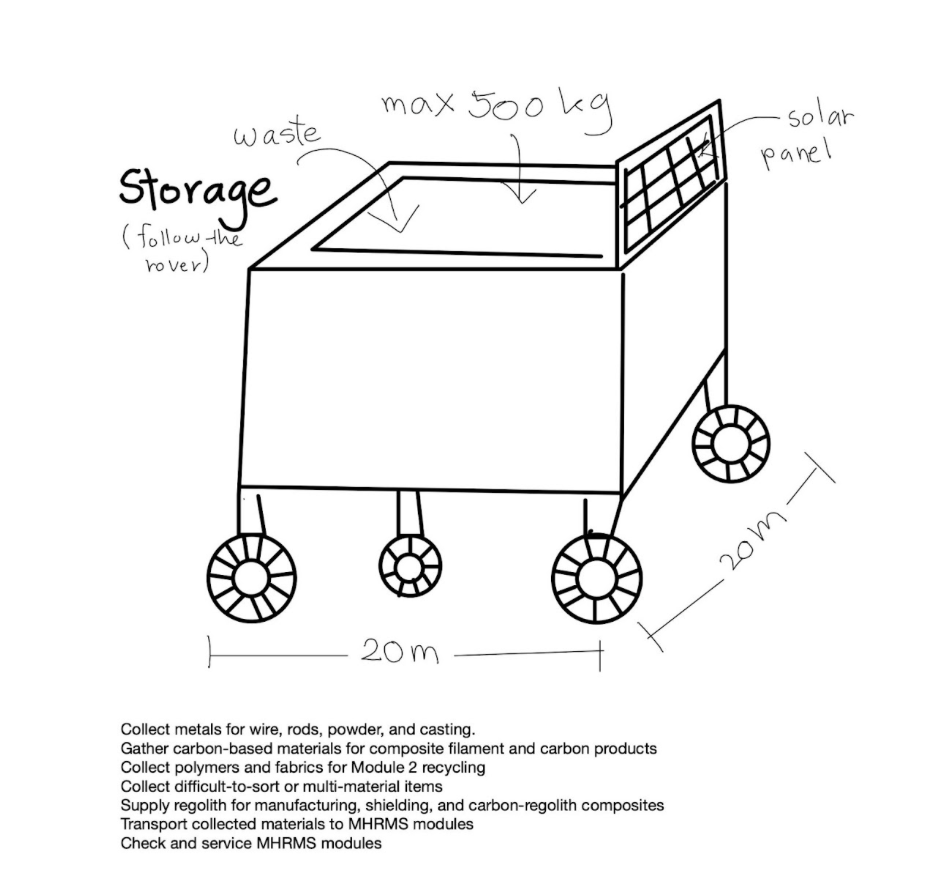
\includegraphics[width=\textwidth]{rover1.png}
        \caption{Rover 1 Docking Mechanism and Carbon Collection System}
        \label{fig:rover1_design}
    \end{minipage}
    \hfill
    \begin{minipage}{0.45\textwidth}
        \centering
        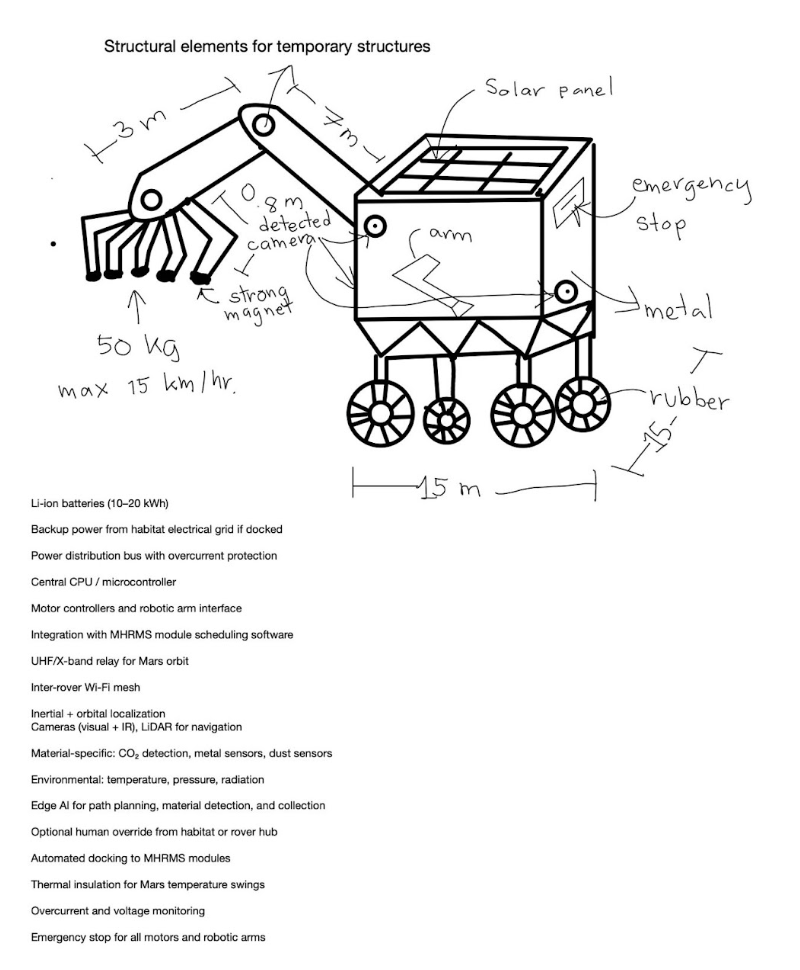
\includegraphics[width=\textwidth]{rover2.png}
        \caption{Rover 4 Separation Bay and Material Processing Unit}
        \label{fig:rover4_design}
    \end{minipage}
\end{figure}

\section{Common Design \& Engineering Specifications}

\subsection{Materials Selection}
\begin{itemize}
    \item \textbf{Chassis:} Aluminum-lithium alloys for strength-to-weight optimization
    \item \textbf{Covers:} Composite panels for durability and thermal management
    \item \textbf{Gripper Surfaces:} Stainless steel for abrasion resistance
    \item \textbf{Protection:} Advanced shielding and coatings for dust abrasion mitigation
\end{itemize}

\subsection{Seals \& Dust Mitigation}
\begin{itemize}
    \item Double-seal approach on all openings for redundancy
    \item Pre-opening purge systems to prevent contamination
    \item Magnetic seals on high-use charge and data points
    \item Comprehensive dust exclusion throughout all systems
\end{itemize}

\subsection{Standardization Protocols}
\begin{itemize}
    \item Identical power/data docking geometry across entire fleet
    \item Interchangeable electronic components and modules
    \item Common software architecture and communication protocols
    \item Unified maintenance and diagnostic interfaces
\end{itemize}

\subsection{Redundancy \& Safety Systems}
\begin{itemize}
    \item Each rover carries minimal emergency toolkit and beacon
    \item Manual tether systems for emergency retrieval
    \item Multiple E-stop locations (remote and physical access)
    \item Thermal cutouts on all heating elements and processing units
    \item Safety interlocks on all material handling systems
\end{itemize}

\subsection{Operational Reliability}
\begin{itemize}
    \item Designed for continuous operation in Mars environment
    \item Radiation-hardened electronics where required
    \item Thermal cycling resilience for extreme temperature variations
    \item Dust tolerance in all moving parts and seals
    \item Maintenance-friendly design for crew servicing
\end{itemize}

\section{Special Controlled Environment Habitat for MHRMS \& Rover Fleet}

\subsection{Mission \& Design Philosophy}

\subsubsection{Mission Statement}
Provide a dedicated, fully controlled habitat for material collection, recycling, processing, manufacturing, and fleet operations on Mars. Ensure high operational efficiency, safety, minimal crew involvement, and expansion potential.

\subsubsection{Design Goals}
\begin{itemize}
    \item Fully modular \& relocatable architecture
    \item Integrated habitat electrical grid powered operations
    \item Closed-loop environmental control (air, water, temperature, dust)
    \item Automated and remote-monitorable systems
    \item Future-proof for additional modules, manufacturing technologies, or new rover types
    \item Maintainable with minimal crew intervention
\end{itemize}

\subsection{Habitat Structural Layout}

\subsubsection{Core Structural Design}

\textbf{Central Spine Module:}
\begin{itemize}
    \item Main access corridor and control hub
    \item Houses central control servers, environmental monitoring, and power distribution
    \item Acts as backbone connecting all modules
\end{itemize}

\textbf{Modular Side Pods:}
\begin{itemize}
    \item Each side pod hosts specific MHRMS modules (1-4) or storage
    \item Docking and maintenance bays at ends for rovers
    \item Pass-through corridors allow robotic and automated transfer between modules
\end{itemize}

\textbf{Construction Specifications:}
\begin{itemize}
    \item Pressurized aluminum-lithium alloy shell with multilayer insulation
    \item Internal vibration dampers for sensitive manufacturing/filtration equipment
    \item Expandable docking rings for new modules or rover types
\end{itemize}

\subsubsection{Zones \& Modules}

\begin{table}[h!]
\centering
\small
\renewcommand{\arraystretch}{1.4}
\setlength{\tabcolsep}{8pt}
\begin{tabular}{p{0.3\textwidth} p{0.65\textwidth}}
\toprule
\textbf{Zone} & \textbf{Purpose and Features} \\
\midrule
MHRMS Processing Pods & 
\begin{itemize}
\setlength\itemsep{0.1em}
\item Modules 1-4 operations
\item Negative-pressure grinding chambers
\item High-temperature melting/extrusion zones
\item Filtration and vapor capture systems
\item Automated material transfer between modules
\end{itemize} \\[1em]

Rover Docking \& Maintenance Bays &
\begin{itemize}
\setlength\itemsep{0.1em}
\item Fleet operations center
\item 1 bay per rover type (7 total)
\item Automated docking, charging, data synchronization
\item Robotic maintenance arms for repairs
\item Sealed transfer ports for material handling
\end{itemize} \\[1em]

Material Storage \& Sorting Pods &
\begin{itemize}
\setlength\itemsep{0.1em}
\item Waste storage and pre-processing
\item Category-based storage (Carbon, Polymers, Metals, Fabrics, Regolith)
\item Climate-controlled for sublimation-sensitive materials
\item Automated conveyors and robotic handling systems
\end{itemize} \\[1em]

Manufacturing Pod &
\begin{itemize}
\setlength\itemsep{0.1em}
\item 3D printing and post-processing
\item FDM plastic/composite printing stations
\item Metal filament and powder printing capabilities
\item CNC machining and finishing equipment
\item Quality control and storage racks for finished products
\end{itemize} \\[1em]

Future Expansion Rings &
\begin{itemize}
\setlength\itemsep{0.1em}
\item Accommodation for future modules
\item Empty docking and pass-through ports
\item Flexible power and environmental interfaces
\item Prewired for robotics or new processing technologies
\end{itemize} \\
\bottomrule
\end{tabular}
\caption{Habitat Zones and Their Functions}
\end{table}
\normalsize

\subsection{Environmental \& Habitat Controls}

\subsubsection{Atmosphere Management}
\begin{itemize}
    \item Pressurized to 101 kPa (Earth standard)
    \item Oxygen/Nitrogen mix maintained at optimal levels
    \item CO\textsubscript{2} scrubbers and VOC filters (linked to Module 1 carbon processing)
    \item HEPA filtration for microplastics and dust control
    \item Airlocks with dust mitigation systems for rover entry/exit
\end{itemize}

\subsubsection{Thermal \& Energy Systems}
\begin{itemize}
    \item Habitat insulation maintains 20°C ±5°C operational temperature
    \item Local heating/cooling for processing modules: 150-1400°C zones as required
    \item Waste heat recycled from high-temperature operations to preheat incoming modules
    \item Phase-change thermal buffers to smooth out Mars sol temperature cycles
    \item Grid-powered with redundancy for each pod
\end{itemize}

\subsubsection{Water \& Humidity Control}
\begin{itemize}
    \item Closed-loop water system for polymer/fabric drying processes
    \item Minimal water consumption design philosophy
    \item Vapor recapture and reuse systems
    \item Humidity maintained at 40-50\% in sensitive manufacturing zones
\end{itemize}

\subsubsection{Dust \& Contamination Control}
\begin{itemize}
    \item Negative-pressure chambers for all grinding and shredding operations
    \item Rover docking systems sealed to prevent dust escape
    \item Automated HEPA and activated carbon filtration in all pods
    \item Contaminants returned to processing streams whenever possible
\end{itemize}

\subsection{Rover Integration}

\subsubsection{Docking Bay Design Features}
\begin{itemize}
    \item Automated charging interface (grid-powered)
    \item Material transfer ports connected to storage pods
    \item Robotic arms for minor repairs and module replacement
    \item Environmental status sensors and operational health monitoring
    \item Designated pathways for autonomous navigation within habitat
\end{itemize}

\subsubsection{Supported Rover Types}
\begin{itemize}
    \item Carbon collector rover
    \item Polymer/Plastic collector rover
    \item Metal collector rover
    \item Composite/Mixed-material collector rover
    \item Regolith/ISRU rover
    \item Storage/Transport rover
    \item Maintenance/Inspection rover
\end{itemize}

\subsection{Workflow (Automated \& Modular)}

\subsubsection{Material Collection Phase}
\begin{itemize}
    \item Rovers gather materials from external environment
    \item Automated docking at designated bays
    \item Material deposition into categorized storage pods
\end{itemize}

\subsubsection{Material Sorting \& Pre-processing}
\begin{itemize}
    \item Automated conveyors and robotic arms sort materials by category
    \item Pre-processing operations: grinding, drying, shredding
    \item Quality assessment and contamination removal
\end{itemize}

\subsubsection{Processing Operations}
\begin{itemize}
    \item Modules 1-3 handle carbon, polymer/fabric, and metal processing
    \item Filament and powder production with quality control
    \item Continuous material flow between processing stages
\end{itemize}

\subsubsection{Manufacturing Operations}
\begin{itemize}
    \item Module 4 manages 3D printing of finished products
    \item Production includes: tools, replacement parts, habitat components
    \item CNC finishing ensures adherence to design tolerances
\end{itemize}

\subsubsection{Rover Maintenance \& Support}
\begin{itemize}
    \item Maintenance/inspection rovers handle minor repairs
    \item Automated monitoring systems detect anomalies
    \item Preventive maintenance scheduling
\end{itemize}

\subsubsection{Future Expansion Capabilities}
\begin{itemize}
    \item New processing modules can be integrated seamlessly
    \item Advanced manufacturing technologies can be added
    \item Expanded storage pods for increased capacity
\end{itemize}

\subsection{Safety \& Redundancy Systems}

\subsubsection{Power Management}
\begin{itemize}
    \item Multiple grid feeds with automatic failover
    \item Redundant power distribution to critical systems
    \item Emergency power reserves for life support systems
\end{itemize}

\subsubsection{Temperature Control}
\begin{itemize}
    \item Thermal alarms and monitoring systems
    \item Interlocked access controls for high-temperature zones
    \item Emergency cooling systems for overheating scenarios
\end{itemize}

\subsubsection{Environmental Protection}
\begin{itemize}
    \item HEPA and activated carbon filtration redundancy
    \item Continuous particulate monitoring
    \item Emergency ventilation and purge systems
\end{itemize}

\subsubsection{Fire Safety}
\begin{itemize}
    \item CO\textsubscript{2} suppression systems for metal or electrical fires
    \item Fire detection and alarm systems throughout habitat
    \item Emergency evacuation protocols and safe zones
\end{itemize}

\subsubsection{Automation \& Monitoring}
\begin{itemize}
    \item System alerts crew for anomalies requiring intervention
    \item Minimal crew involvement in routine operations
    \item Remote monitoring capability from main habitat
\end{itemize}

\subsubsection{Maintenance Protocols}
\begin{itemize}
    \item Robotic module swaps to minimize downtime
    \item Regular inspection schedules
    \item Predictive maintenance based on operational data
\end{itemize}

\subsection{Future-Ready Features}

\subsubsection{Modular Expansion Capability}
\begin{itemize}
    \item Prewired docking rings for new MHRMS modules
    \item Accommodation for future rover types and technologies
    \item Scalable power and environmental interfaces
\end{itemize}

\subsubsection{Advanced Manufacturing Integration}
\begin{itemize}
    \item Support for multi-material 3D printers
    \item Capability for biocomposites processing
    \item Integration of regolith-based ceramics and glass manufacturing
\end{itemize}

\subsubsection{Robotic Autonomy Enhancement}
\begin{itemize}
    \item Future AI systems for full material flow management
    \item Autonomous decision-making for operational optimization
    \item Reduced dependency on crew oversight
\end{itemize}

\subsubsection{Distributed Manufacturing}
\begin{itemize}
    \item Mobile MHRMS pods deployable across Mars surface
    \item Satellite manufacturing outposts
    \item Emergency repair capabilities at remote sites
\end{itemize}

\subsubsection{Colony Scale Integration}
\begin{itemize}
    \item Habitat clusters connected via modular corridors
    \item Large-scale Mars settlement infrastructure
    \item Industrial-scale recycling and manufacturing capabilities
\end{itemize}

\subsection{Summary}

The Advanced Modular Mars MHRMS Habitat represents a comprehensive solution for sustainable operations on Mars, characterized by:

\begin{itemize}
    \item \textbf{Dedicated Focus:} Fully optimized for MHRMS processing and rover fleet operations
    \item \textbf{Future-Ready Design:} Modular, expandable, and adaptable to emerging technologies
    \item \textbf{Safe \& Efficient Operations:} Closed-loop environmental systems with minimal crew involvement
    \item \textbf{Scalable Architecture:} Capable of growth with additional modules, rovers, and advanced manufacturing systems
    \item \textbf{Full Integration:} Seamless material flow from collection through processing to manufacturing and storage
\end{itemize}

\section{Conclusion}

This integrated recycling-to-manufacturing system transforms Mars habitat waste—including fabrics, food packaging, foam, EVA materials, aluminum structures, and carbon from CO2 extraction—into valuable 3D printing feedstock and finished products. The modular design is powered by the habitat's electrical grid and optimized for Mars conditions while maintaining crew safety and environmental responsibility.

\textbf{Key Innovation:} Leveraging Mars's unique environment (thin atmosphere, low pressure) as advantages rather than obstacles, while processing a comprehensive range of waste materials into useful end products.

\textbf{Mission Impact:} Enables long-duration Mars missions by creating a closed-loop resource economy, reducing Earth dependency, and providing on-demand manufacturing capability for tools, utensils, storage containers, interior habitat outfitting, and habitat expansion.

\textbf{Ready for Development:} All core technologies proven; integration and Mars-specific optimization required before deployment.

\section{MHRMS System Summary}

The Mars Habitat Recycling-to-Manufacturing System (MHRMS) represents a comprehensive, integrated solution for sustainable resource management on Mars. This system transforms the challenge of waste accumulation into an opportunity for resource independence and manufacturing capability.

\subsection{Core System Overview}

The MHRMS is a modular, grid-powered system designed for Mars habitats to transform all types of waste—including plastics, metals, fabrics, composites, and carbon byproducts—into usable materials for 3D printing and manufacturing. By integrating recycling with production, it enables long-term sustainability, reduces dependency on Earth resupply, and supports habitat expansion.

\subsection{Four Core Processing Modules}

\begin{table}[h!]
\centering
\small
\renewcommand{\arraystretch}{1.4}
\setlength{\tabcolsep}{8pt}
\begin{tabular}{p{0.22\textwidth} p{0.35\textwidth} p{0.38\textwidth}}
\toprule
\textbf{Module} & \textbf{Primary Function} & \textbf{Key Outputs} \\
\midrule
Carbon Processing Station & Converts carbon waste into composite materials & Composite filament, activated carbon filters, graphite components, radiation shielding blocks \\[0.5em]

Polymer Recycling Station & Processes plastics and fabrics into reusable materials & PE/PP filament, EVA blends, polyester/nylon filaments, mixed-polymer materials \\[0.5em]

Metal Processing Station & Recycles metallic waste into manufacturing feedstock & Metal wire filament, metal powder, direct-cast tools and components \\[0.5em]

Integrated Manufacturing Hub & Transforms recycled materials into finished products & Tools, habitat components, life support parts, scientific instruments, EVA equipment \\
\bottomrule
\end{tabular}
\caption{MHRMS Core Processing Modules and Their Functions}
\end{table}
\normalsize

\subsection{Mars-Optimized Design Features}

\subsubsection{Environmental Adaptation}
\begin{itemize}
    \item \textbf{Thermal Management:} Designed for Mars temperature extremes (-153°C to 20°C) with insulated chambers and waste heat recovery
    \item \textbf{Dust Mitigation:} Sealed systems and HEPA filtration prevent Martian dust contamination
    \item \textbf{Low Pressure Optimization:} Leverages Mars' thin atmosphere for efficient cooling and processing
    \item \textbf{Mars Sol Synchronization:} Operations calibrated to 24.6-hour Martian day for optimal efficiency
\end{itemize}

\subsubsection{Operational Efficiency}
\begin{itemize}
    \item \textbf{Minimal Crew Time:} Requires only 2-3 hours daily crew involvement through extensive automation
    \item \textbf{High Recovery Rates:} Achieves 85-95\% material recovery across all waste categories
    \item \textbf{Continuous Operation:} Automated processes continue during crew sleep cycles
    \item \textbf{Quick Maintenance:} Modular design enables rapid component replacement and repairs
\end{itemize}

\subsection{Material Input Categories}

The system processes six comprehensive waste categories:

\begin{itemize}
    \item \textbf{Carbon Materials:} CO\textsubscript{2} extraction byproducts, activated carbon filters, carbon composites
    \item \textbf{Polymers/Plastics:} Packaging materials, EVA waste, nitrile gloves, resealable bags
    \item \textbf{Fabrics:} Clothing, wipes, disinfectant materials (cotton, polyester, nylon)
    \item \textbf{Food Packaging:} Rehydratable pouches, drink containers, overwrap materials
    \item \textbf{Metals:} Broken tools, structural components, electronics casings, wire scraps
    \item \textbf{Composites:} Multi-layer materials, adhesive-bonded assemblies, fabric-backed composites
\end{itemize}

\subsection{Integrated Rover Fleet Support}

The MHRMS is complemented by a specialized rover fleet that ensures efficient material collection and system maintenance:

\begin{itemize}
    \item \textbf{7 Specialized Rovers:} Carbon collector, polymer collector, metal collector, composite separator, regolith excavator, transport hauler, maintenance rover
    \item \textbf{Automated Workflow:} From collection to processing to manufacturing with minimal human intervention
    \item \textbf{Standardized Design:} Shared electronics compartment for easy maintenance and part interchangeability
\end{itemize}

\subsection{Key Performance Metrics}

\begin{table}[h!]
\centering
\small
\renewcommand{\arraystretch}{1.3}
\setlength{\tabcolsep}{10pt}
\begin{tabular}{p{0.4\textwidth} p{0.25\textwidth} p{0.3\textwidth}}
\toprule
\textbf{Metric} & \textbf{Performance} & \textbf{Impact} \\
\midrule
Daily Processing Capacity & 15-25 kg & Supports 8-person crew waste generation \\
Material Recovery Rate & 85-96\% & Minimal waste residue \\
Earth Resupply Reduction & 60-80\% & Significant cost savings \\
System Mass & ~720 kg & Transport-efficient modular design \\
Power Consumption & 7.5-14.5 kW & Compatible with habitat power systems \\
Crew Time Requirement & 2-3 hours/day & Minimal operational burden \\
\bottomrule
\end{tabular}
\caption{MHRMS Key Performance Indicators}
\end{table}
\normalsize

\subsection{Strategic Advantages}

\subsubsection{Mission Sustainability}
\begin{itemize}
    \item Creates closed-loop resource economy on Mars
    \item Eliminates waste accumulation and environmental contamination
    \item Enables indefinite mission extension without additional launches
    \item Supports permanent settlement through continuous resource cycling
\end{itemize}

\subsubsection{Economic Benefits}
\begin{itemize}
    \item Reduces launch costs by \$10,000 per kilogram of material recycled
    \item System pays for itself within 2-3 months of operation
    \item Enables cost-effective mission scaling and colony expansion
    \item Minimizes dependency on expensive Earth resupply missions
\end{itemize}

\subsubsection{Operational Flexibility}
\begin{itemize}
    \item Processes unexpected waste streams and mission byproducts
    \item Creates custom tools and parts on-demand for mission needs
    \item Supports emergency repairs and contingency operations
    \item Adaptable to new materials and manufacturing requirements
\end{itemize}

\subsection{Future Development and Scaling}

\subsubsection{Near-Term Enhancements}
\begin{itemize}
    \item Integration of regolith processing for ceramics and glass production
    \item Advanced multi-material 3D printing capabilities
    \item Enhanced AI and automation for reduced crew involvement
    \item Expanded material library including biocomposites
\end{itemize}

\subsubsection{Long-Term Vision}
\begin{itemize}
    \item Colony-scale operations supporting 100+ inhabitants
    \item Distributed manufacturing networks across Mars surface
    \item Industrial-scale material processing and production
    \item Integration with global Mars resource economy
\end{itemize}

\subsection{Conclusion}

In essence, the Mars Habitat Recycling-to-Manufacturing System transforms the fundamental challenge of waste management into a strategic advantage for Mars exploration and settlement. By converting waste into valuable materials and functional components, MHRMS enables:

\begin{itemize}
    \item \textbf{True Self-Sufficiency:} Mars habitats can maintain and expand themselves using local resources
    \item \textbf{Sustainable Operations:} Closed-loop systems prevent environmental contamination and resource depletion
    \item \textbf{Mission Resilience:} On-demand manufacturing capability supports unexpected needs and repairs
    \item \textbf{Economic Viability:} Dramatic reduction in Earth dependency makes long-term presence feasible
    \item \textbf{Colony Foundation:} The system provides the manufacturing backbone for permanent human settlement
\end{itemize}

The MHRMS represents not just a waste management solution, but a fundamental enabling technology for humanity's future as a multi-planetary species. It embodies the principle of living off the land while maintaining environmental stewardship, ensuring that our presence on Mars is sustainable, scalable, and scientifically productive.

\noindent\textbf{System Status:} Ready for development with proven core technologies; requires integration and Mars-specific optimization before deployment.

\begin{thebibliography}{9}

\bibitem{howe2010}
Howe, A. Scott; Howard, Robert. 2010. ``Dual use of packaging on the moon: Logistics-2-Living.'' \textit{AIAA 40th International Conference on Environmental Systems}, Barcelona, Spain, July 11-15, 2010. JPL Open Repository. \url{https://hdl.handle.net/2014/45116}

\bibitem{mgs1}
MGS-1 Mars Global Simulant. \url{https://sciences.ucf.edu/class/simulant_marsglobal/}

\bibitem{nasa_facts}
NASA Mars Facts. \url{https://science.nasa.gov/mars/facts/}

\bibitem{nasa_trash}
NASA Trash-to-Gas and Trash-to-Supply Gas research. \url{https://ntrs.nasa.gov/api/citations/20130011661/downloads/20130011661.pdf}

\end{thebibliography}

\end{document}